\chapter{Range queries}

\index{range query}
\index{sum query}
\index{minimum query}
\index{maximum query}

In this chapter, we discuss data structures
that allow us to efficiently answer range queries.
In a \key{range query}, we are given two indices
to an array, and our task is to calculate some
value based on the elements between the given indices.
Typical range queries are:
\begin{itemize}
\item \key{sum query}: calculate the sum of elements
\item \key{minimum query}: find the smallest element
\item \key{maximum query}: find the largest element
\end{itemize}
For example, consider the range $[4,7]$ in the following array:
\begin{center}
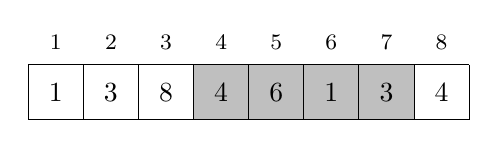
\begin{tikzpicture}[scale=0.7]
\fill[color=lightgray] (3,0) rectangle (7,1);
\draw (0,0) grid (8,1);

\node at (0.5,0.5) {$1$};
\node at (1.5,0.5) {$3$};
\node at (2.5,0.5) {$8$};
\node at (3.5,0.5) {$4$};
\node at (4.5,0.5) {$6$};
\node at (5.5,0.5) {$1$};
\node at (6.5,0.5) {$3$};
\node at (7.5,0.5) {$4$};

\footnotesize
\node at (0.5,1.4) {$1$};
\node at (1.5,1.4) {$2$};
\node at (2.5,1.4) {$3$};
\node at (3.5,1.4) {$4$};
\node at (4.5,1.4) {$5$};
\node at (5.5,1.4) {$6$};
\node at (6.5,1.4) {$7$};
\node at (7.5,1.4) {$8$};
\end{tikzpicture}
\end{center}
In this range, the sum of elements is $4+6+1+3=16$,
the minimum element is 1 and the maximum element is 6.

A simple way to process range queries is to
go through all elements in the range.
For example, the following function \texttt{sum}
calculates the sum of elements in a range
$[a,b]$ of an array $t$:

\begin{lstlisting}
int sum(int a, int b) {
    int s = 0;
    for (int i = a; i <= b; i++) {
        s += t[i];
    }
    return s;
}
\end{lstlisting}

The above function works in $O(n)$ time,
where $n$ is the number of elements in the array.
Thus, we can process $q$ queries in $O(nq)$
time using the function.
However, if both $n$ and $q$ are large, this approach
is slow, and it turns out that there are
ways to process range queries much more efficiently.

\section{Static array queries}

We first focus on a situation where
the array is \key{static}, i.e.,
the elements are never modified between the queries.
In this case, it suffices to construct
a static data structure that tells us
the answer for any possible query.

\subsubsection{Sum queries}

\index{prefix sum array}

It turns out that we can easily process
sum queries on a static array,
because we can use a data structure called
a \key{prefix sum array}.
Each value in such an array equals
the sum of values in the original array up to that position.

For example, consider the following array:
\begin{center}
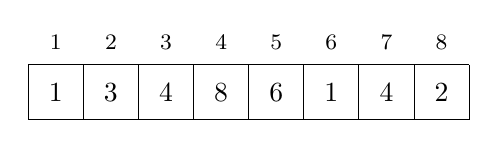
\begin{tikzpicture}[scale=0.7]
%\fill[color=lightgray] (3,0) rectangle (7,1);
\draw (0,0) grid (8,1);

\node at (0.5,0.5) {$1$};
\node at (1.5,0.5) {$3$};
\node at (2.5,0.5) {$4$};
\node at (3.5,0.5) {$8$};
\node at (4.5,0.5) {$6$};
\node at (5.5,0.5) {$1$};
\node at (6.5,0.5) {$4$};
\node at (7.5,0.5) {$2$};

\footnotesize
\node at (0.5,1.4) {$1$};
\node at (1.5,1.4) {$2$};
\node at (2.5,1.4) {$3$};
\node at (3.5,1.4) {$4$};
\node at (4.5,1.4) {$5$};
\node at (5.5,1.4) {$6$};
\node at (6.5,1.4) {$7$};
\node at (7.5,1.4) {$8$};
\end{tikzpicture}
\end{center}
The corresponding prefix sum array is as follows:
\begin{center}
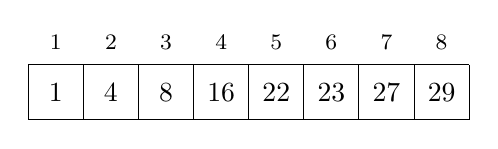
\begin{tikzpicture}[scale=0.7]
%\fill[color=lightgray] (3,0) rectangle (7,1);
\draw (0,0) grid (8,1);

\node at (0.5,0.5) {$1$};
\node at (1.5,0.5) {$4$};
\node at (2.5,0.5) {$8$};
\node at (3.5,0.5) {$16$};
\node at (4.5,0.5) {$22$};
\node at (5.5,0.5) {$23$};
\node at (6.5,0.5) {$27$};
\node at (7.5,0.5) {$29$};


\footnotesize
\node at (0.5,1.4) {$1$};
\node at (1.5,1.4) {$2$};
\node at (2.5,1.4) {$3$};
\node at (3.5,1.4) {$4$};
\node at (4.5,1.4) {$5$};
\node at (5.5,1.4) {$6$};
\node at (6.5,1.4) {$7$};
\node at (7.5,1.4) {$8$};
\end{tikzpicture}
\end{center}
Let $\textrm{sum}(a,b)$ denote the sum of elements
in the range $[a,b]$.
Since the prefix sum array contains all values
of the form $\textrm{sum}(1,k)$,
we can calculate any value of
$\textrm{sum}(a,b)$ in $O(1)$ time, because
\[ \textrm{sum}(a,b) = \textrm{sum}(1,b) - \textrm{sum}(1,a-1).\]
By defining $\textrm{sum}(1,0)=0$,
the above formula also holds when $a=1$.

For example, consider the range $[4,7]$:
\begin{center}
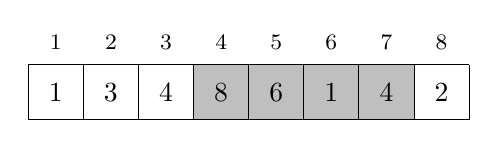
\begin{tikzpicture}[scale=0.7]
\fill[color=lightgray] (3,0) rectangle (7,1);
\draw (0,0) grid (8,1);

\node at (0.5,0.5) {$1$};
\node at (1.5,0.5) {$3$};
\node at (2.5,0.5) {$4$};
\node at (3.5,0.5) {$8$};
\node at (4.5,0.5) {$6$};
\node at (5.5,0.5) {$1$};
\node at (6.5,0.5) {$4$};
\node at (7.5,0.5) {$2$};

\footnotesize
\node at (0.5,1.4) {$1$};
\node at (1.5,1.4) {$2$};
\node at (2.5,1.4) {$3$};
\node at (3.5,1.4) {$4$};
\node at (4.5,1.4) {$5$};
\node at (5.5,1.4) {$6$};
\node at (6.5,1.4) {$7$};
\node at (7.5,1.4) {$8$};
\end{tikzpicture}
\end{center}
The sum in the range is $8+6+1+4=19$.
This sum can be calculated using
two values in the prefix sum array:
\begin{center}
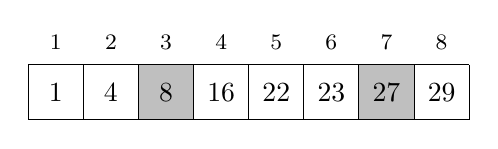
\begin{tikzpicture}[scale=0.7]
\fill[color=lightgray] (2,0) rectangle (3,1);
\fill[color=lightgray] (6,0) rectangle (7,1);
\draw (0,0) grid (8,1);

\node at (0.5,0.5) {$1$};
\node at (1.5,0.5) {$4$};
\node at (2.5,0.5) {$8$};
\node at (3.5,0.5) {$16$};
\node at (4.5,0.5) {$22$};
\node at (5.5,0.5) {$23$};
\node at (6.5,0.5) {$27$};
\node at (7.5,0.5) {$29$};


\footnotesize
\node at (0.5,1.4) {$1$};
\node at (1.5,1.4) {$2$};
\node at (2.5,1.4) {$3$};
\node at (3.5,1.4) {$4$};
\node at (4.5,1.4) {$5$};
\node at (5.5,1.4) {$6$};
\node at (6.5,1.4) {$7$};
\node at (7.5,1.4) {$8$};
\end{tikzpicture}
\end{center}
Thus, the sum in the range $[4,7]$ is $27-8=19$.

It is also possible to generalize this idea
to higher dimensions.
For example, we can construct a two-dimensional
prefix sum array that can be used for calculating
the sum of any rectangular subarray in $O(1)$ time.
Each value in such an array is the sum of a subarray
that begins at the upper-left corner of the array.

\begin{samepage}
The following picture illustrates the idea:
\begin{center}
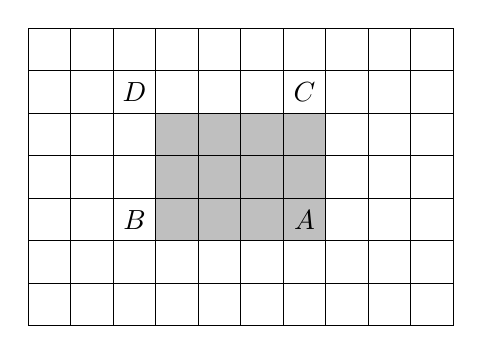
\begin{tikzpicture}[scale=0.54]
\draw[fill=lightgray] (3,2) rectangle (7,5);
\draw (0,0) grid (10,7);
%\draw[line width=2pt] (3,2) rectangle (7,5);
\node[anchor=center] at (6.5, 2.5) {$A$};
\node[anchor=center] at (2.5, 2.5) {$B$};
\node[anchor=center] at (6.5, 5.5) {$C$};
\node[anchor=center] at (2.5, 5.5) {$D$};
\end{tikzpicture}
\end{center}
\end{samepage}

The sum of the gray subarray can be calculated
using the formula
\[S(A) - S(B) - S(C) + S(D),\]
where $S(X)$ denotes the sum of a rectangular
subarray from the upper-left corner
to the position of $X$.

\subsubsection{Minimum queries}

Next we will see how we can
process range minimum queries in $O(1)$ time
after an $O(n \log n)$ time preprocessing using \index{sparse table}
a data structure called a \key{sparse table}\footnote{The
sparse table structure was introduced in \cite{ben00}.
There are also more sophisticated techniques \cite{fis06} where
the preprocessing time of the array is only $O(n)$, but such algorithms
are not needed in competitive programming.}.
Note that minimum and maximum queries can always
be processed using similar techniques,
so it suffices to focus on minimum queries.

Let $\textrm{rmq}(a,b)$ (''range minimum query'')
denote the minimum element in the range $[a,b]$.
The idea is to precalculate all values of $\textrm{rmq}(a,b)$
where $b-a+1$, the length of the range, is a power of two.
For example, for the array

\begin{center}
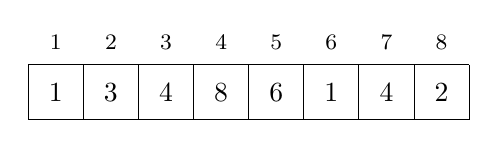
\begin{tikzpicture}[scale=0.7]
\draw (0,0) grid (8,1);

\node at (0.5,0.5) {$1$};
\node at (1.5,0.5) {$3$};
\node at (2.5,0.5) {$4$};
\node at (3.5,0.5) {$8$};
\node at (4.5,0.5) {$6$};
\node at (5.5,0.5) {$1$};
\node at (6.5,0.5) {$4$};
\node at (7.5,0.5) {$2$};

\footnotesize
\node at (0.5,1.4) {$1$};
\node at (1.5,1.4) {$2$};
\node at (2.5,1.4) {$3$};
\node at (3.5,1.4) {$4$};
\node at (4.5,1.4) {$5$};
\node at (5.5,1.4) {$6$};
\node at (6.5,1.4) {$7$};
\node at (7.5,1.4) {$8$};
\end{tikzpicture}
\end{center}
the following values will be calculated:

\begin{center}
\begin{tabular}{ccc}

\begin{tabular}{ccc}
$a$ & $b$ & $\textrm{rmq}(a,b)$ \\
\hline
1 & 1 & 1 \\
2 & 2 & 3 \\
3 & 3 & 4 \\
4 & 4 & 8 \\
5 & 5 & 6 \\
6 & 6 & 1 \\
7 & 7 & 4 \\
8 & 8 & 2 \\
\end{tabular}

&

\begin{tabular}{ccc}
$a$ & $b$ & $\textrm{rmq}(a,b)$ \\
\hline
1 & 2 & 1 \\
2 & 3 & 3 \\
3 & 4 & 4 \\
4 & 5 & 6 \\
5 & 6 & 1 \\
6 & 7 & 1 \\
7 & 8 & 2 \\
\\
\end{tabular}

&

\begin{tabular}{ccc}
$a$ & $b$ & $\textrm{rmq}(a,b)$ \\
\hline
1 & 4 & 1 \\
2 & 5 & 3 \\
3 & 6 & 1 \\
4 & 7 & 1 \\
5 & 8 & 1 \\
1 & 8 & 1 \\
\\
\\
\end{tabular}

\end{tabular}
\end{center}

The number of precalculated values is $O(n \log n)$,
because there are $O(\log n)$ range lengths
that are powers of two.
In addition, the values can be calculated efficiently
using the recursive formula
\[\textrm{rmq}(a,b) = \min(\textrm{rmq}(a,a+w-1),\textrm{rmq}(a+w,b)),\]
where $b-a+1$ is a power of two and $w=(b-a+1)/2$.
Calculating all those values takes $O(n \log n)$ time.

After this, any value of $\textrm{rmq}(a,b)$ can be calculated
in $O(1)$ time as a minimum of two precalculated values.
Let $k$ be the largest power of two that does not exceed $b-a+1$.
We can calculate the value of $\textrm{rmq}(a,b)$ using the formula
\[\textrm{rmq}(a,b) = \min(\textrm{rmq}(a,a+k-1),\textrm{rmq}(b-k+1,b)).\]
In the above formula, the range $[a,b]$ is represented
as the union of the ranges $[a,a+k-1]$ and $[b-k+1,b]$, both of length $k$.

As an example, consider the range $[2,7]$:
\begin{center}
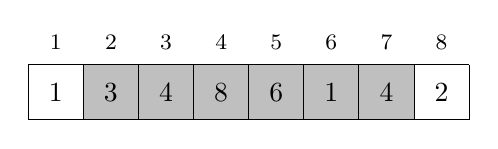
\begin{tikzpicture}[scale=0.7]
\fill[color=lightgray] (1,0) rectangle (7,1);
\draw (0,0) grid (8,1);

\node at (0.5,0.5) {$1$};
\node at (1.5,0.5) {$3$};
\node at (2.5,0.5) {$4$};
\node at (3.5,0.5) {$8$};
\node at (4.5,0.5) {$6$};
\node at (5.5,0.5) {$1$};
\node at (6.5,0.5) {$4$};
\node at (7.5,0.5) {$2$};

\footnotesize
\node at (0.5,1.4) {$1$};
\node at (1.5,1.4) {$2$};
\node at (2.5,1.4) {$3$};
\node at (3.5,1.4) {$4$};
\node at (4.5,1.4) {$5$};
\node at (5.5,1.4) {$6$};
\node at (6.5,1.4) {$7$};
\node at (7.5,1.4) {$8$};
\end{tikzpicture}
\end{center}
The length of the range is 6,
and the largest power of two that does
not exceed 6 is 4.
Thus the range $[2,7]$ is
the union of the ranges $[2,5]$ and $[4,7]$:
\begin{center}
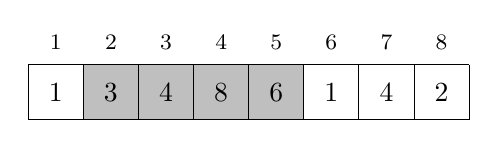
\begin{tikzpicture}[scale=0.7]
\fill[color=lightgray] (1,0) rectangle (5,1);
\draw (0,0) grid (8,1);

\node at (0.5,0.5) {$1$};
\node at (1.5,0.5) {$3$};
\node at (2.5,0.5) {$4$};
\node at (3.5,0.5) {$8$};
\node at (4.5,0.5) {$6$};
\node at (5.5,0.5) {$1$};
\node at (6.5,0.5) {$4$};
\node at (7.5,0.5) {$2$};

\footnotesize
\node at (0.5,1.4) {$1$};
\node at (1.5,1.4) {$2$};
\node at (2.5,1.4) {$3$};
\node at (3.5,1.4) {$4$};
\node at (4.5,1.4) {$5$};
\node at (5.5,1.4) {$6$};
\node at (6.5,1.4) {$7$};
\node at (7.5,1.4) {$8$};
\end{tikzpicture}
\end{center}
\begin{center}
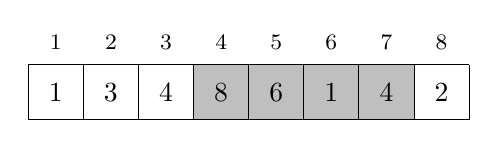
\begin{tikzpicture}[scale=0.7]
\fill[color=lightgray] (3,0) rectangle (7,1);
\draw (0,0) grid (8,1);

\node at (0.5,0.5) {$1$};
\node at (1.5,0.5) {$3$};
\node at (2.5,0.5) {$4$};
\node at (3.5,0.5) {$8$};
\node at (4.5,0.5) {$6$};
\node at (5.5,0.5) {$1$};
\node at (6.5,0.5) {$4$};
\node at (7.5,0.5) {$2$};


\footnotesize
\node at (0.5,1.4) {$1$};
\node at (1.5,1.4) {$2$};
\node at (2.5,1.4) {$3$};
\node at (3.5,1.4) {$4$};
\node at (4.5,1.4) {$5$};
\node at (5.5,1.4) {$6$};
\node at (6.5,1.4) {$7$};
\node at (7.5,1.4) {$8$};
\end{tikzpicture}
\end{center}
Since $\textrm{rmq}(2,5)=3$ and $\textrm{rmq}(4,7)=1$,
we can conclude that $\textrm{rmq}(2,7)=1$.

\section{Binary indexed trees}

\index{binary indexed tree}
\index{Fenwick tree}

A \key{binary indexed tree} or \key{Fenwick tree}\footnote{The
binary indexed tree structure was presented by P. M. Fenwick in 1994 \cite{fen94}.}
can be seen as a dynamic version of a prefix sum array.
This data structure supports two $O(\log n)$ time operations:
calculating the sum of elements in a range
and modifying the value of an element.

The advantage of a binary indexed tree is
that it allows us to efficiently update
the array elements between the sum queries.
This would not be possible using a prefix sum array,
because after each update, we should build the
whole array again in $O(n)$ time.

\subsubsection{Structure}

A binary indexed tree can be represented as an array
where the value at position $x$ 
equals the sum of elements in the range $[x-k+1,x]$,
where $k$ is the largest power of two that divides $x$.
For example, if $x=6$, then $k=2$, because 2 divides 6
but 4 does not divide 6.

\begin{samepage}
For example, consider the following array:
\begin{center}
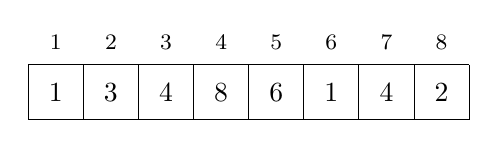
\begin{tikzpicture}[scale=0.7]
\draw (0,0) grid (8,1);

\node at (0.5,0.5) {$1$};
\node at (1.5,0.5) {$3$};
\node at (2.5,0.5) {$4$};
\node at (3.5,0.5) {$8$};
\node at (4.5,0.5) {$6$};
\node at (5.5,0.5) {$1$};
\node at (6.5,0.5) {$4$};
\node at (7.5,0.5) {$2$};

\footnotesize
\node at (0.5,1.4) {$1$};
\node at (1.5,1.4) {$2$};
\node at (2.5,1.4) {$3$};
\node at (3.5,1.4) {$4$};
\node at (4.5,1.4) {$5$};
\node at (5.5,1.4) {$6$};
\node at (6.5,1.4) {$7$};
\node at (7.5,1.4) {$8$};
\end{tikzpicture}
\end{center}
\end{samepage}
\begin{samepage}
The corresponding binary indexed tree is as follows:
\begin{center}
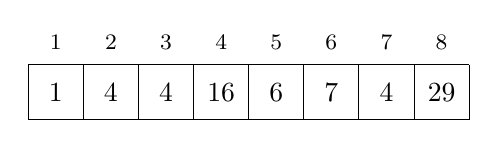
\begin{tikzpicture}[scale=0.7]
\draw (0,0) grid (8,1);

\node at (0.5,0.5) {$1$};
\node at (1.5,0.5) {$4$};
\node at (2.5,0.5) {$4$};
\node at (3.5,0.5) {$16$};
\node at (4.5,0.5) {$6$};
\node at (5.5,0.5) {$7$};
\node at (6.5,0.5) {$4$};
\node at (7.5,0.5) {$29$};

\footnotesize
\node at (0.5,1.4) {$1$};
\node at (1.5,1.4) {$2$};
\node at (2.5,1.4) {$3$};
\node at (3.5,1.4) {$4$};
\node at (4.5,1.4) {$5$};
\node at (5.5,1.4) {$6$};
\node at (6.5,1.4) {$7$};
\node at (7.5,1.4) {$8$};
\end{tikzpicture}
\end{center}
\end{samepage}

For example, the value at position 6
in the binary indexed tree is 7,
because the sum of elements in the range $[5,6]$
of the array is $6+1=7$.

The following picture shows more clearly
how each value in the binary indexed tree
corresponds to a range in the array:

\begin{center}
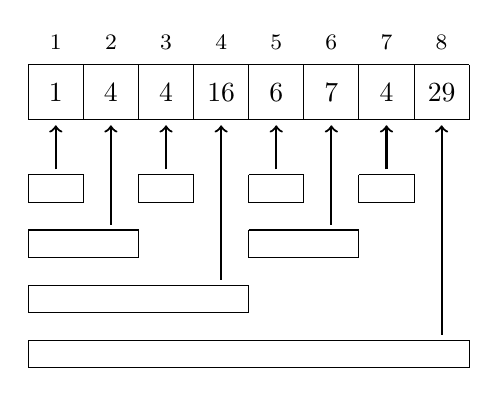
\begin{tikzpicture}[scale=0.7]
%\fill[color=lightgray] (3,0) rectangle (7,1);
\draw (0,0) grid (8,1);

\node at (0.5,0.5) {$1$};
\node at (1.5,0.5) {$4$};
\node at (2.5,0.5) {$4$};
\node at (3.5,0.5) {$16$};
\node at (4.5,0.5) {$6$};
\node at (5.5,0.5) {$7$};
\node at (6.5,0.5) {$4$};
\node at (7.5,0.5) {$29$};

\footnotesize
\node at (0.5,1.4) {$1$};
\node at (1.5,1.4) {$2$};
\node at (2.5,1.4) {$3$};
\node at (3.5,1.4) {$4$};
\node at (4.5,1.4) {$5$};
\node at (5.5,1.4) {$6$};
\node at (6.5,1.4) {$7$};
\node at (7.5,1.4) {$8$};

\draw[->,thick] (0.5,-0.9) -- (0.5,-0.1);
\draw[->,thick] (2.5,-0.9) -- (2.5,-0.1);
\draw[->,thick] (4.5,-0.9) -- (4.5,-0.1);
\draw[->,thick] (6.5,-0.9) -- (6.5,-0.1);
\draw[->,thick] (1.5,-1.9) -- (1.5,-0.1);
\draw[->,thick] (5.5,-1.9) -- (5.5,-0.1);
\draw[->,thick] (3.5,-2.9) -- (3.5,-0.1);
\draw[->,thick] (7.5,-3.9) -- (7.5,-0.1);

\draw (0,-1) -- (1,-1) -- (1,-1.5) -- (0,-1.5) -- (0,-1);
\draw (2,-1) -- (3,-1) -- (3,-1.5) -- (2,-1.5) -- (2,-1);
\draw (4,-1) -- (5,-1) -- (5,-1.5) -- (4,-1.5) -- (4,-1);
\draw (6,-1) -- (7,-1) -- (7,-1.5) -- (6,-1.5) -- (6,-1);
\draw (0,-2) -- (2,-2) -- (2,-2.5) -- (0,-2.5) -- (0,-2);
\draw (4,-2) -- (6,-2) -- (6,-2.5) -- (4,-2.5) -- (4,-2);
\draw (0,-3) -- (4,-3) -- (4,-3.5) -- (0,-3.5) -- (0,-3);
\draw (0,-4) -- (8,-4) -- (8,-4.5) -- (0,-4.5) -- (0,-4);
\end{tikzpicture}
\end{center}

\subsubsection{Sum queries}

The values in the binary indexed tree
can be used to efficiently calculate
the sum of elements in any range $[1,k]$,
because such a range
can be divided into $O(\log n)$ ranges
whose sums are available in the binary indexed tree.

For example, the range $[1,7]$ corresponds to
the following values:
\begin{center}
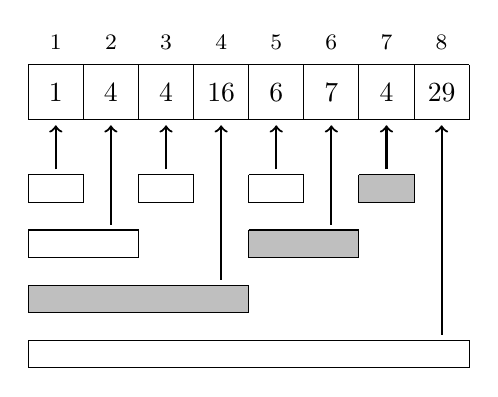
\begin{tikzpicture}[scale=0.7]
%\fill[color=lightgray] (3,0) rectangle (7,1);
\draw (0,0) grid (8,1);

\node at (0.5,0.5) {$1$};
\node at (1.5,0.5) {$4$};
\node at (2.5,0.5) {$4$};
\node at (3.5,0.5) {$16$};
\node at (4.5,0.5) {$6$};
\node at (5.5,0.5) {$7$};
\node at (6.5,0.5) {$4$};
\node at (7.5,0.5) {$29$};

\footnotesize
\node at (0.5,1.4) {$1$};
\node at (1.5,1.4) {$2$};
\node at (2.5,1.4) {$3$};
\node at (3.5,1.4) {$4$};
\node at (4.5,1.4) {$5$};
\node at (5.5,1.4) {$6$};
\node at (6.5,1.4) {$7$};
\node at (7.5,1.4) {$8$};

\draw[->,thick] (0.5,-0.9) -- (0.5,-0.1);
\draw[->,thick] (2.5,-0.9) -- (2.5,-0.1);
\draw[->,thick] (4.5,-0.9) -- (4.5,-0.1);
\draw[->,thick] (6.5,-0.9) -- (6.5,-0.1);
\draw[->,thick] (1.5,-1.9) -- (1.5,-0.1);
\draw[->,thick] (5.5,-1.9) -- (5.5,-0.1);
\draw[->,thick] (3.5,-2.9) -- (3.5,-0.1);
\draw[->,thick] (7.5,-3.9) -- (7.5,-0.1);

\draw (0,-1) -- (1,-1) -- (1,-1.5) -- (0,-1.5) -- (0,-1);
\draw (2,-1) -- (3,-1) -- (3,-1.5) -- (2,-1.5) -- (2,-1);
\draw (4,-1) -- (5,-1) -- (5,-1.5) -- (4,-1.5) -- (4,-1);
\draw[fill=lightgray] (6,-1) -- (7,-1) -- (7,-1.5) -- (6,-1.5) -- (6,-1);
\draw (0,-2) -- (2,-2) -- (2,-2.5) -- (0,-2.5) -- (0,-2);
\draw[fill=lightgray] (4,-2) -- (6,-2) -- (6,-2.5) -- (4,-2.5) -- (4,-2);
\draw[fill=lightgray] (0,-3) -- (4,-3) -- (4,-3.5) -- (0,-3.5) -- (0,-3);
\draw (0,-4) -- (8,-4) -- (8,-4.5) -- (0,-4.5) -- (0,-4);
\end{tikzpicture}
\end{center}

Hence, the sum of elements in the range $[1,7]$ is $16+7+4=27$.

To calculate the sum of elements in any range $[a,b]$,
we can use the same trick that we used with prefix sum arrays:
\[ \textrm{sum}(a,b) = \textrm{sum}(1,b) - \textrm{sum}(1,a-1).\]
Also in this case, only $O(\log n)$ values are needed.

\subsubsection{Array updates}

When a value in the array changes,
several values in the binary indexed tree should be updated.
For example, if the element at position 3 changes,
the sums of the following ranges change:
\begin{center}
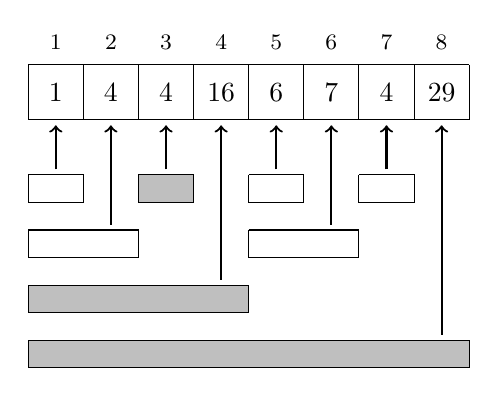
\begin{tikzpicture}[scale=0.7]
%\fill[color=lightgray] (3,0) rectangle (7,1);
\draw (0,0) grid (8,1);

\node at (0.5,0.5) {$1$};
\node at (1.5,0.5) {$4$};
\node at (2.5,0.5) {$4$};
\node at (3.5,0.5) {$16$};
\node at (4.5,0.5) {$6$};
\node at (5.5,0.5) {$7$};
\node at (6.5,0.5) {$4$};
\node at (7.5,0.5) {$29$};

\footnotesize
\node at (0.5,1.4) {$1$};
\node at (1.5,1.4) {$2$};
\node at (2.5,1.4) {$3$};
\node at (3.5,1.4) {$4$};
\node at (4.5,1.4) {$5$};
\node at (5.5,1.4) {$6$};
\node at (6.5,1.4) {$7$};
\node at (7.5,1.4) {$8$};

\draw[->,thick] (0.5,-0.9) -- (0.5,-0.1);
\draw[->,thick] (2.5,-0.9) -- (2.5,-0.1);
\draw[->,thick] (4.5,-0.9) -- (4.5,-0.1);
\draw[->,thick] (6.5,-0.9) -- (6.5,-0.1);
\draw[->,thick] (1.5,-1.9) -- (1.5,-0.1);
\draw[->,thick] (5.5,-1.9) -- (5.5,-0.1);
\draw[->,thick] (3.5,-2.9) -- (3.5,-0.1);
\draw[->,thick] (7.5,-3.9) -- (7.5,-0.1);

\draw (0,-1) -- (1,-1) -- (1,-1.5) -- (0,-1.5) -- (0,-1);
\draw[fill=lightgray] (2,-1) -- (3,-1) -- (3,-1.5) -- (2,-1.5) -- (2,-1);
\draw (4,-1) -- (5,-1) -- (5,-1.5) -- (4,-1.5) -- (4,-1);
\draw (6,-1) -- (7,-1) -- (7,-1.5) -- (6,-1.5) -- (6,-1);
\draw (0,-2) -- (2,-2) -- (2,-2.5) -- (0,-2.5) -- (0,-2);
\draw (4,-2) -- (6,-2) -- (6,-2.5) -- (4,-2.5) -- (4,-2);
\draw[fill=lightgray] (0,-3) -- (4,-3) -- (4,-3.5) -- (0,-3.5) -- (0,-3);
\draw[fill=lightgray] (0,-4) -- (8,-4) -- (8,-4.5) -- (0,-4.5) -- (0,-4);
\end{tikzpicture}
\end{center}

Since each array element belongs to $O(\log n)$
ranges in the binary indexed tree,
it suffices to update $O(\log n)$ values.


\subsubsection{Implementation}

The operations of a binary indexed tree can be implemented
in an elegant and efficient way using bit operations.
The key fact needed is that $k \& -k$
isolates the last one bit of a number $k$.
For example, $26 \& -26=2$ because the number $26$
corresponds to 11010 and the number $2$ corresponds to 10.

It turns out that when processing a sum query,
the position $k$ in the binary indexed tree needs to be
decreased by $k \& -k$ at every step,
and when updating the array,
the position $k$ needs to be increased by $k \& -k$ at every step.

Suppose that the binary indexed tree is stored in an array \texttt{b}.
The following function calculates
the sum of elements in a range $[1,k]$:
\begin{lstlisting}
int sum(int k) {
    int s = 0;
    while (k >= 1) {
        s += b[k];
        k -= k&-k;
    }
    return s;
}
\end{lstlisting}

The following function increases the value
of the element at position $k$ by $x$
($x$ can be positive or negative):
\begin{lstlisting}
void add(int k, int x) {
    while (k <= n) {
        b[k] += x;
        k += k&-k;
    }
}
\end{lstlisting}

The time complexity of both the functions is
$O(\log n)$, because the functions access $O(\log n)$
values in the binary indexed tree, and each move
to the next position
takes $O(1)$ time using bit operations.

\section{Segment trees}

\index{segment tree}

A \key{segment tree}\footnote{The origin of this structure is unknown.
The bottom-up-implementation in this chapter corresponds to
the implementation in \cite{sta06}.} is a data structure
that supports two operations:
processing a range query and
modifying an element in the array.
Segment trees can support
sum queries, minimum and maximum queries and many other
queries so that both operations work in $O(\log n)$ time.

Compared to a binary indexed tree,
the advantage of a segment tree is that it is
a more general data structure.
While binary indexed trees only support
sum queries, segment trees also support other queries.
On the other hand, a segment tree requires more
memory and is a bit more difficult to implement.

\subsubsection{Structure}

A segment tree is a binary tree
such that the nodes on the bottom level of the tree
correspond to the array elements,
and the other nodes
contain information needed for processing range queries.

Throughout the section, we assume that the size
of the array is a power of two and zero-based
indexing is used, because it is convenient to build
a segment tree for such an array.
If the size of the array is not a power of two,
we can always append extra elements to it.

We will first discuss segment trees that support sum queries.
As an example, consider the following array:
\begin{center}
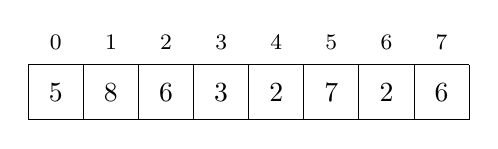
\begin{tikzpicture}[scale=0.7]
\draw (0,0) grid (8,1);

\node at (0.5,0.5) {$5$};
\node at (1.5,0.5) {$8$};
\node at (2.5,0.5) {$6$};
\node at (3.5,0.5) {$3$};
\node at (4.5,0.5) {$2$};
\node at (5.5,0.5) {$7$};
\node at (6.5,0.5) {$2$};
\node at (7.5,0.5) {$6$};

\footnotesize
\node at (0.5,1.4) {$0$};
\node at (1.5,1.4) {$1$};
\node at (2.5,1.4) {$2$};
\node at (3.5,1.4) {$3$};
\node at (4.5,1.4) {$4$};
\node at (5.5,1.4) {$5$};
\node at (6.5,1.4) {$6$};
\node at (7.5,1.4) {$7$};
\end{tikzpicture}
\end{center}
The corresponding segment tree is as follows:
\begin{center}
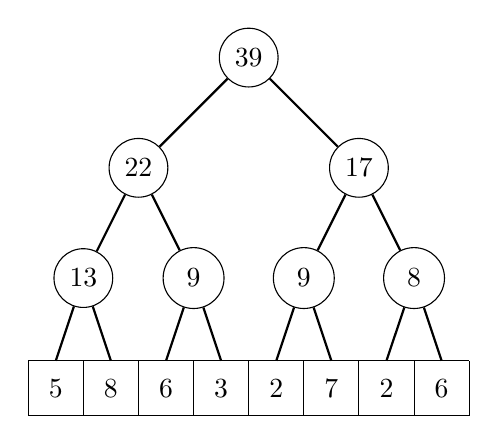
\begin{tikzpicture}[scale=0.7]
\draw (0,0) grid (8,1);

\node[anchor=center] at (0.5, 0.5) {5};
\node[anchor=center] at (1.5, 0.5) {8};
\node[anchor=center] at (2.5, 0.5) {6};
\node[anchor=center] at (3.5, 0.5) {3};
\node[anchor=center] at (4.5, 0.5) {2};
\node[anchor=center] at (5.5, 0.5) {7};
\node[anchor=center] at (6.5, 0.5) {2};
\node[anchor=center] at (7.5, 0.5) {6};

\node[draw, circle] (a) at (1,2.5) {13};
\path[draw,thick,-] (a) -- (0.5,1);
\path[draw,thick,-] (a) -- (1.5,1);
\node[draw, circle,minimum size=22pt] (b) at (3,2.5) {9};
\path[draw,thick,-] (b) -- (2.5,1);
\path[draw,thick,-] (b) -- (3.5,1);
\node[draw, circle,minimum size=22pt] (c) at (5,2.5) {9};
\path[draw,thick,-] (c) -- (4.5,1);
\path[draw,thick,-] (c) -- (5.5,1);
\node[draw, circle,minimum size=22pt] (d) at (7,2.5) {8};
\path[draw,thick,-] (d) -- (6.5,1);
\path[draw,thick,-] (d) -- (7.5,1);

\node[draw, circle] (i) at (2,4.5) {22};
\path[draw,thick,-] (i) -- (a);
\path[draw,thick,-] (i) -- (b);
\node[draw, circle] (j) at (6,4.5) {17};
\path[draw,thick,-] (j) -- (c);
\path[draw,thick,-] (j) -- (d);

\node[draw, circle] (m) at (4,6.5) {39};
\path[draw,thick,-] (m) -- (i);
\path[draw,thick,-] (m) -- (j);
\end{tikzpicture}
\end{center}

Each internal node in the segment tree contains
information about a range of size $2^k$
in the original array.
In the above tree, the value of each internal
node is the sum of the corresponding array elements,
and it can be calculated as the sum of
the values of its left and right child node.

\subsubsection{Range queries}

The sum of elements in a given range
can be calculated as a sum of values in the segment tree.
For example, consider the following range:
\begin{center}
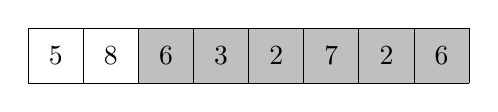
\begin{tikzpicture}[scale=0.7]
\fill[color=gray!50] (2,0) rectangle (8,1);
\draw (0,0) grid (8,1);

\node[anchor=center] at (0.5, 0.5) {5};
\node[anchor=center] at (1.5, 0.5) {8};
\node[anchor=center] at (2.5, 0.5) {6};
\node[anchor=center] at (3.5, 0.5) {3};
\node[anchor=center] at (4.5, 0.5) {2};
\node[anchor=center] at (5.5, 0.5) {7};
\node[anchor=center] at (6.5, 0.5) {2};
\node[anchor=center] at (7.5, 0.5) {6};
% 
% \footnotesize
% \node at (0.5,1.4) {$1$};
% \node at (1.5,1.4) {$2$};
% \node at (2.5,1.4) {$3$};
% \node at (3.5,1.4) {$4$};
% \node at (4.5,1.4) {$5$};
% \node at (5.5,1.4) {$6$};
% \node at (6.5,1.4) {$7$};
% \node at (7.5,1.4) {$8$};
\end{tikzpicture}
\end{center}
The sum of elements in the range is
$6+3+2+7+2+6=26$.
The following two nodes in the tree
correspond to the range:
\begin{center}
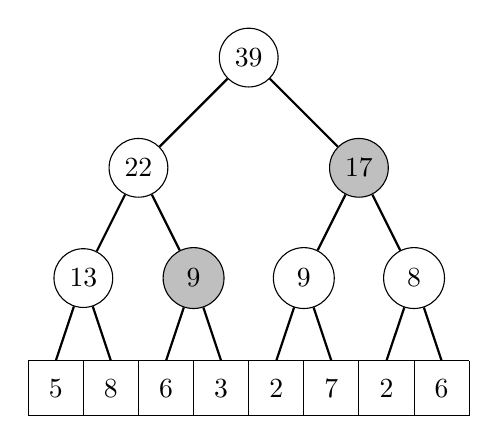
\begin{tikzpicture}[scale=0.7]
\draw (0,0) grid (8,1);

\node[anchor=center] at (0.5, 0.5) {5};
\node[anchor=center] at (1.5, 0.5) {8};
\node[anchor=center] at (2.5, 0.5) {6};
\node[anchor=center] at (3.5, 0.5) {3};
\node[anchor=center] at (4.5, 0.5) {2};
\node[anchor=center] at (5.5, 0.5) {7};
\node[anchor=center] at (6.5, 0.5) {2};
\node[anchor=center] at (7.5, 0.5) {6};

\node[draw, circle] (a) at (1,2.5) {13};
\path[draw,thick,-] (a) -- (0.5,1);
\path[draw,thick,-] (a) -- (1.5,1);
\node[draw, circle,fill=gray!50,minimum size=22pt] (b) at (3,2.5) {9};
\path[draw,thick,-] (b) -- (2.5,1);
\path[draw,thick,-] (b) -- (3.5,1);
\node[draw, circle,minimum size=22pt] (c) at (5,2.5) {9};
\path[draw,thick,-] (c) -- (4.5,1);
\path[draw,thick,-] (c) -- (5.5,1);
\node[draw, circle,minimum size=22pt] (d) at (7,2.5) {8};
\path[draw,thick,-] (d) -- (6.5,1);
\path[draw,thick,-] (d) -- (7.5,1);

\node[draw, circle] (i) at (2,4.5) {22};
\path[draw,thick,-] (i) -- (a);
\path[draw,thick,-] (i) -- (b);
\node[draw, circle,fill=gray!50] (j) at (6,4.5) {17};
\path[draw,thick,-] (j) -- (c);
\path[draw,thick,-] (j) -- (d);

\node[draw, circle] (m) at (4,6.5) {39};
\path[draw,thick,-] (m) -- (i);
\path[draw,thick,-] (m) -- (j);
\end{tikzpicture}
\end{center}
Thus, the sum of elements in the range is $9+17=26$.

When the sum is calculated using nodes
that are located as high as possible in the tree,
at most two nodes on each level
of the tree are needed.
Hence, the total number of nodes
is only $O(\log n)$.

\subsubsection{Array updates}

When an element in the array changes,
we should update all nodes in the tree
whose value depends on the element.
This can be done by traversing the path
from the element to the top node
and updating the nodes along the path.

\begin{samepage}
The following picture shows which nodes in the segment tree
change if the element 7 in the array changes.

\begin{center}
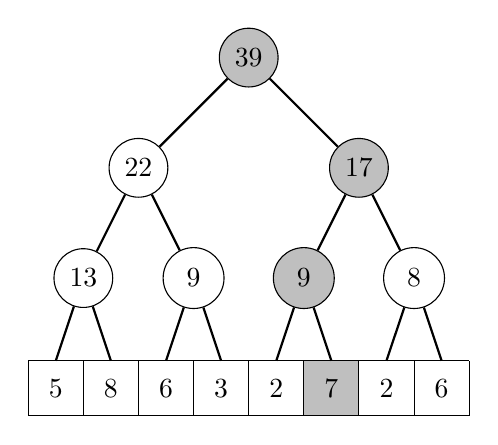
\begin{tikzpicture}[scale=0.7]
\fill[color=gray!50] (5,0) rectangle (6,1);
\draw (0,0) grid (8,1);

\node[anchor=center] at (0.5, 0.5) {5};
\node[anchor=center] at (1.5, 0.5) {8};
\node[anchor=center] at (2.5, 0.5) {6};
\node[anchor=center] at (3.5, 0.5) {3};
\node[anchor=center] at (4.5, 0.5) {2};
\node[anchor=center] at (5.5, 0.5) {7};
\node[anchor=center] at (6.5, 0.5) {2};
\node[anchor=center] at (7.5, 0.5) {6};

\node[draw, circle] (a) at (1,2.5) {13};
\path[draw,thick,-] (a) -- (0.5,1);
\path[draw,thick,-] (a) -- (1.5,1);
\node[draw, circle,minimum size=22pt] (b) at (3,2.5) {9};
\path[draw,thick,-] (b) -- (2.5,1);
\path[draw,thick,-] (b) -- (3.5,1);
\node[draw, circle,minimum size=22pt,fill=gray!50] (c) at (5,2.5) {9};
\path[draw,thick,-] (c) -- (4.5,1);
\path[draw,thick,-] (c) -- (5.5,1);
\node[draw, circle,minimum size=22pt] (d) at (7,2.5) {8};
\path[draw,thick,-] (d) -- (6.5,1);
\path[draw,thick,-] (d) -- (7.5,1);

\node[draw, circle] (i) at (2,4.5) {22};
\path[draw,thick,-] (i) -- (a);
\path[draw,thick,-] (i) -- (b);
\node[draw, circle,fill=gray!50] (j) at (6,4.5) {17};
\path[draw,thick,-] (j) -- (c);
\path[draw,thick,-] (j) -- (d);

\node[draw, circle,fill=gray!50] (m) at (4,6.5) {39};
\path[draw,thick,-] (m) -- (i);
\path[draw,thick,-] (m) -- (j);
\end{tikzpicture}
\end{center}
\end{samepage}

The path from bottom to top
always consists of $O(\log n)$ nodes,
so each update changes $O(\log n)$ nodes in the tree.

\subsubsection{Storing the tree}

A segment tree can be stored in an array
of $2N$ elements where $N$ is a power of two.
Such a tree corresponds to an array
indexed from $0$ to $N-1$.

In the segment tree array,
the element at position 1
corresponds to the top node of the tree,
the elements at positions 2 and 3 correspond to
the second level of the tree, and so on.
Finally, the elements at positions $N \ldots 2N-1$
correspond to the bottom level of the tree, i.e.,
the elements of the original array.

For example, the segment tree
\begin{center}
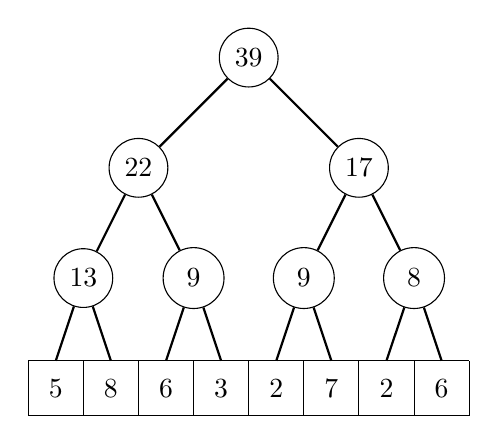
\begin{tikzpicture}[scale=0.7]
\draw (0,0) grid (8,1);

\node[anchor=center] at (0.5, 0.5) {5};
\node[anchor=center] at (1.5, 0.5) {8};
\node[anchor=center] at (2.5, 0.5) {6};
\node[anchor=center] at (3.5, 0.5) {3};
\node[anchor=center] at (4.5, 0.5) {2};
\node[anchor=center] at (5.5, 0.5) {7};
\node[anchor=center] at (6.5, 0.5) {2};
\node[anchor=center] at (7.5, 0.5) {6};

\node[draw, circle] (a) at (1,2.5) {13};
\path[draw,thick,-] (a) -- (0.5,1);
\path[draw,thick,-] (a) -- (1.5,1);
\node[draw, circle,minimum size=22pt] (b) at (3,2.5) {9};
\path[draw,thick,-] (b) -- (2.5,1);
\path[draw,thick,-] (b) -- (3.5,1);
\node[draw, circle,minimum size=22pt] (c) at (5,2.5) {9};
\path[draw,thick,-] (c) -- (4.5,1);
\path[draw,thick,-] (c) -- (5.5,1);
\node[draw, circle,minimum size=22pt] (d) at (7,2.5) {8};
\path[draw,thick,-] (d) -- (6.5,1);
\path[draw,thick,-] (d) -- (7.5,1);

\node[draw, circle] (i) at (2,4.5) {22};
\path[draw,thick,-] (i) -- (a);
\path[draw,thick,-] (i) -- (b);
\node[draw, circle] (j) at (6,4.5) {17};
\path[draw,thick,-] (j) -- (c);
\path[draw,thick,-] (j) -- (d);

\node[draw, circle] (m) at (4,6.5) {39};
\path[draw,thick,-] (m) -- (i);
\path[draw,thick,-] (m) -- (j);
\end{tikzpicture}
\end{center}
can be stored as follows ($N=8$):
\begin{center}
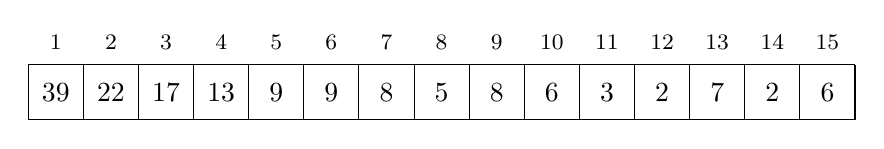
\begin{tikzpicture}[scale=0.7]
%\fill[color=lightgray] (3,0) rectangle (7,1);
\draw (0,0) grid (15,1);

\node at (0.5,0.5) {$39$};
\node at (1.5,0.5) {$22$};
\node at (2.5,0.5) {$17$};
\node at (3.5,0.5) {$13$};
\node at (4.5,0.5) {$9$};
\node at (5.5,0.5) {$9$};
\node at (6.5,0.5) {$8$};
\node at (7.5,0.5) {$5$};
\node at (8.5,0.5) {$8$};
\node at (9.5,0.5) {$6$};
\node at (10.5,0.5) {$3$};
\node at (11.5,0.5) {$2$};
\node at (12.5,0.5) {$7$};
\node at (13.5,0.5) {$2$};
\node at (14.5,0.5) {$6$};

\footnotesize
\node at (0.5,1.4) {$1$};
\node at (1.5,1.4) {$2$};
\node at (2.5,1.4) {$3$};
\node at (3.5,1.4) {$4$};
\node at (4.5,1.4) {$5$};
\node at (5.5,1.4) {$6$};
\node at (6.5,1.4) {$7$};
\node at (7.5,1.4) {$8$};
\node at (8.5,1.4) {$9$};
\node at (9.5,1.4) {$10$};
\node at (10.5,1.4) {$11$};
\node at (11.5,1.4) {$12$};
\node at (12.5,1.4) {$13$};
\node at (13.5,1.4) {$14$};
\node at (14.5,1.4) {$15$};
\end{tikzpicture}
\end{center}
Using this representation,
for a node at position $k$,
\begin{itemize}
\item the parent node is at position $\lfloor k/2 \rfloor$,
\item the left child node is at position $2k$, and
\item the right child node is at position $2k+1$.
\end{itemize}
% Note that this implies that the index of a node
% is even if it is a left child and odd if it is a right child.

\subsubsection{Functions}

Assume that the segment tree is stored
in an array \texttt{p}.
The following function
calculates the sum of elements in a range $[a,b]$:

\begin{lstlisting}
int sum(int a, int b) {
    a += N; b += N;
    int s = 0;
    while (a <= b) {
        if (a%2 == 1) s += p[a++];
        if (b%2 == 0) s += p[b--];
        a /= 2; b /= 2;
    }
    return s;
}
\end{lstlisting}

The function starts at the bottom of the tree
and moves one level up at each step.
Initially, the range $[a+N,b+N]$ corresponds
to the range $[a,b]$ in the original array.
At each step, the function adds the value of
the left and right node to the sum
if their parent nodes do not belong to the range.
This process continues, until the sum of the
range has been calculated.

The following function increases the value
of the element at position $k$ by $x$:

\begin{lstlisting}
void add(int k, int x) {
    k += N;
    p[k] += x;
    for (k /= 2; k >= 1; k /= 2) {
        p[k] = p[2*k]+p[2*k+1];
    }
}
\end{lstlisting}
First the function updates the element
at the bottom level of the tree.
After this, the function updates the values of all
internal nodes in the tree, until it reaches
the top node of the tree.

Both above functions work
in $O(\log n)$ time, because a segment tree
of $n$ elements consists of $O(\log n)$ levels,
and the operations move one level forward in the tree at each step.

\subsubsection{Other queries}

Segment trees can support any queries
as long as we can divide a range into two parts,
calculate the answer for both parts
and then efficiently combine the answers.
Examples of such queries are
minimum and maximum, greatest common divisor,
and bit operations and, or and xor.

\begin{samepage}
For example, the following segment tree
supports minimum queries:

\begin{center}
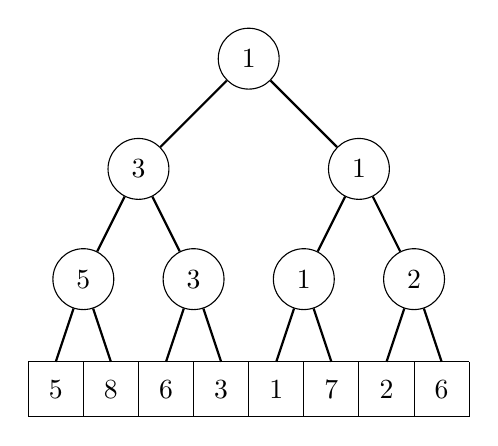
\begin{tikzpicture}[scale=0.7]
\draw (0,0) grid (8,1);

\node[anchor=center] at (0.5, 0.5) {5};
\node[anchor=center] at (1.5, 0.5) {8};
\node[anchor=center] at (2.5, 0.5) {6};
\node[anchor=center] at (3.5, 0.5) {3};
\node[anchor=center] at (4.5, 0.5) {1};
\node[anchor=center] at (5.5, 0.5) {7};
\node[anchor=center] at (6.5, 0.5) {2};
\node[anchor=center] at (7.5, 0.5) {6};

\node[draw, circle,minimum size=22pt] (a) at (1,2.5) {5};
\path[draw,thick,-] (a) -- (0.5,1);
\path[draw,thick,-] (a) -- (1.5,1);
\node[draw, circle,minimum size=22pt] (b) at (3,2.5) {3};
\path[draw,thick,-] (b) -- (2.5,1);
\path[draw,thick,-] (b) -- (3.5,1);
\node[draw, circle,minimum size=22pt] (c) at (5,2.5) {1};
\path[draw,thick,-] (c) -- (4.5,1);
\path[draw,thick,-] (c) -- (5.5,1);
\node[draw, circle,minimum size=22pt] (d) at (7,2.5) {2};
\path[draw,thick,-] (d) -- (6.5,1);
\path[draw,thick,-] (d) -- (7.5,1);

\node[draw, circle,minimum size=22pt] (i) at (2,4.5) {3};
\path[draw,thick,-] (i) -- (a);
\path[draw,thick,-] (i) -- (b);
\node[draw, circle,minimum size=22pt] (j) at (6,4.5) {1};
\path[draw,thick,-] (j) -- (c);
\path[draw,thick,-] (j) -- (d);

\node[draw, circle,minimum size=22pt] (m) at (4,6.5) {1};
\path[draw,thick,-] (m) -- (i);
\path[draw,thick,-] (m) -- (j);
\end{tikzpicture}
\end{center}
\end{samepage}

In this segment tree, every node in the tree
contains the smallest element in the corresponding
range of the array.
The top node of the tree contains the smallest
element in the whole array.
The operations can be implemented like previously,
but instead of sums, minima are calculated.

\subsubsection{Binary search in a tree}

The structure of the segment tree allows us
to use binary search for finding elements in the array.
For example, if the tree supports minimum queries,
we can find the position of the smallest
element in $O(\log n)$ time.

For example, in the following tree the
smallest element 1 can be found
by traversing a path downwards from the top node:

\begin{center}
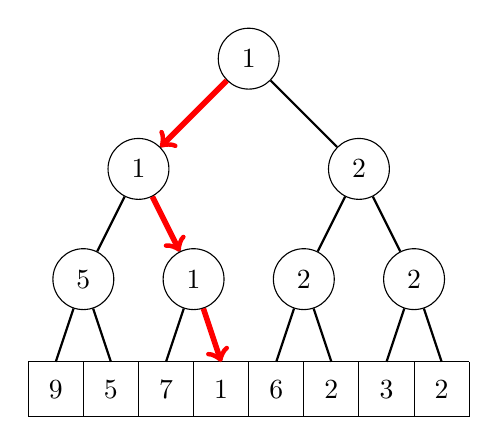
\begin{tikzpicture}[scale=0.7]
\draw (8,0) grid (16,1);

\node[anchor=center] at (8.5, 0.5) {9};
\node[anchor=center] at (9.5, 0.5) {5};
\node[anchor=center] at (10.5, 0.5) {7};
\node[anchor=center] at (11.5, 0.5) {1};
\node[anchor=center] at (12.5, 0.5) {6};
\node[anchor=center] at (13.5, 0.5) {2};
\node[anchor=center] at (14.5, 0.5) {3};
\node[anchor=center] at (15.5, 0.5) {2};

%\node[anchor=center] at (1,2.5) {13};

\node[draw, circle,minimum size=22pt] (e) at (9,2.5) {5};
\path[draw,thick,-] (e) -- (8.5,1);
\path[draw,thick,-] (e) -- (9.5,1);
\node[draw, circle,minimum size=22pt] (f) at (11,2.5) {1};
\path[draw,thick,-] (f) -- (10.5,1);
\path[draw,thick,-] (f) -- (11.5,1);
\node[draw, circle,minimum size=22pt] (g) at (13,2.5) {2};
\path[draw,thick,-] (g) -- (12.5,1);
\path[draw,thick,-] (g) -- (13.5,1);
\node[draw, circle,minimum size=22pt] (h) at (15,2.5) {2};
\path[draw,thick,-] (h) -- (14.5,1);
\path[draw,thick,-] (h) -- (15.5,1);

\node[draw, circle,minimum size=22pt] (k) at (10,4.5) {1};
\path[draw,thick,-] (k) -- (e);
\path[draw,thick,-] (k) -- (f);
\node[draw, circle,minimum size=22pt] (l) at (14,4.5) {2};
\path[draw,thick,-] (l) -- (g);
\path[draw,thick,-] (l) -- (h);

\node[draw, circle,minimum size=22pt] (n) at (12,6.5) {1};
\path[draw,thick,-] (n) -- (k);
\path[draw,thick,-] (n) -- (l);


\path[draw=red,thick,->,line width=2pt] (n) -- (k);
\path[draw=red,thick,->,line width=2pt] (k) -- (f);
\path[draw=red,thick,->,line width=2pt] (f) -- (11.5,1);
\end{tikzpicture}
\end{center}

\section{Additional techniques}

\subsubsection{Index compression}

A limitation in data structures that
are built upon an array is that
the elements are indexed using
consecutive integers.
Difficulties arise when large indices
are needed.
For example, if we wish to use the index $10^9$,
the array should contain $10^9$
elements which would require too much memory.

\index{index compression}

However, we can often bypass this limitation
by using \key{index compression},
where the original indices are replaced
with indices $1,2,3,$ etc.
This can be done if we know all the indices
needed during the algorithm beforehand.

The idea is to replace each original index $x$
with $p(x)$ where $p$ is a function that
compresses the indices.
We require that the order of the indices
does not change, so if $a<b$, then $p(a)<p(b)$.
This allows us to conviently perform queries
even if the indices are compressed.

For example, if the original indices are
$555$, $10^9$ and $8$, the new indices are:

\[
\begin{array}{lcl}
p(8) & = & 1 \\
p(555) & = & 2 \\
p(10^9) & = & 3 \\
\end{array}
\]

\subsubsection{Range updates}

So far, we have implemented data structures
that support range queries and updates
of single values.
Let us now consider an opposite situation,
where we should update ranges and
retrieve single values.
We focus on an operation that increases all
elements in a range $[a,b]$ by $x$.

\index{difference array}

Surprisingly, we can use the data structures
presented in this chapter also in this situation.
To do this, we build a \key{difference array}
for the array.
In such an array, each value indicates
the difference between two consecutive values
in the original array.
Thus, the original array is the
prefix sum array of the
difference array.
For example, consider the following array:

\begin{center}
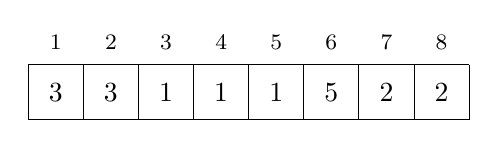
\begin{tikzpicture}[scale=0.7]
\draw (0,0) grid (8,1);

\node at (0.5,0.5) {$3$};
\node at (1.5,0.5) {$3$};
\node at (2.5,0.5) {$1$};
\node at (3.5,0.5) {$1$};
\node at (4.5,0.5) {$1$};
\node at (5.5,0.5) {$5$};
\node at (6.5,0.5) {$2$};
\node at (7.5,0.5) {$2$};


\footnotesize
\node at (0.5,1.4) {$1$};
\node at (1.5,1.4) {$2$};
\node at (2.5,1.4) {$3$};
\node at (3.5,1.4) {$4$};
\node at (4.5,1.4) {$5$};
\node at (5.5,1.4) {$6$};
\node at (6.5,1.4) {$7$};
\node at (7.5,1.4) {$8$};
\end{tikzpicture}
\end{center}

The difference array for the above array is as follows:
\begin{center}
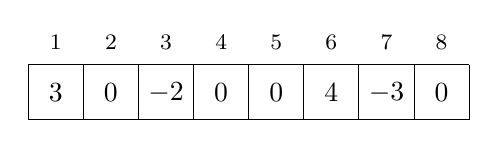
\begin{tikzpicture}[scale=0.7]
\draw (0,0) grid (8,1);

\node at (0.5,0.5) {$3$};
\node at (1.5,0.5) {$0$};
\node at (2.5,0.5) {$-2$};
\node at (3.5,0.5) {$0$};
\node at (4.5,0.5) {$0$};
\node at (5.5,0.5) {$4$};
\node at (6.5,0.5) {$-3$};
\node at (7.5,0.5) {$0$};


\footnotesize
\node at (0.5,1.4) {$1$};
\node at (1.5,1.4) {$2$};
\node at (2.5,1.4) {$3$};
\node at (3.5,1.4) {$4$};
\node at (4.5,1.4) {$5$};
\node at (5.5,1.4) {$6$};
\node at (6.5,1.4) {$7$};
\node at (7.5,1.4) {$8$};
\end{tikzpicture}
\end{center}

For example, the value 5 at position 6 in the original array
corresponds to the sum $3-2+4=5$.

The advantage of the difference array is
that we can update a range
in the original array by changing just
two elements in the difference array.
For example, if we want to 
increase the elements in the range $2 \ldots 5$ by 5,
it suffices to increase the value at position 2 by 5
and decrease the value at position 6 by 5.
The result is as follows:

\begin{center}
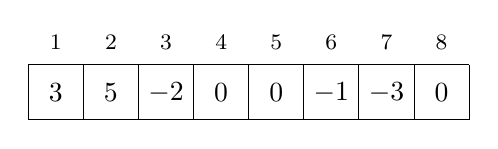
\begin{tikzpicture}[scale=0.7]
\draw (0,0) grid (8,1);

\node at (0.5,0.5) {$3$};
\node at (1.5,0.5) {$5$};
\node at (2.5,0.5) {$-2$};
\node at (3.5,0.5) {$0$};
\node at (4.5,0.5) {$0$};
\node at (5.5,0.5) {$-1$};
\node at (6.5,0.5) {$-3$};
\node at (7.5,0.5) {$0$};

\footnotesize
\node at (0.5,1.4) {$1$};
\node at (1.5,1.4) {$2$};
\node at (2.5,1.4) {$3$};
\node at (3.5,1.4) {$4$};
\node at (4.5,1.4) {$5$};
\node at (5.5,1.4) {$6$};
\node at (6.5,1.4) {$7$};
\node at (7.5,1.4) {$8$};
\end{tikzpicture}
\end{center}

More generally, to increase the elements
in a range $[a,b]$ by $x$,
we increase the value at position $a$ by $x$
and decrease the value at position $b+1$ by $x$.
Thus, it is only needed to update single values
and process sum queries,
so we can use a binary indexed tree or a segment tree.

A more difficult problem is to support both
range queries and range updates.
In Chapter 28 we will see that even this is possible.



